\documentclass[9pt]{beamer}

%!TEX root = ../notas_de_clase.tex

%preamble

 
\usepackage[letterpaper, portrait, margin=0.8in]{geometry}
%language
\usepackage[spanish,es-nodecimaldot]{babel}
\usepackage[utf8]{inputenc}
\usepackage{apacite}



%packages
\usepackage[Algoritmo]{algorithm}
\usepackage{algorithmicx}
\usepackage[noend]{algpseudocode}
\usepackage{mathtools}
\setlength {\marginparwidth }{2cm}
\usepackage{todonotes}
\usepackage{amsbsy}
\usepackage{amssymb}
\usepackage{amsmath,bm}

\usepackage{xcolor}
\providecommand{\red}[1]{\textcolor{red}{\text{#1}}}
\providecommand{\blue}[1]{\textcolor{blue}{\text{#1}}}
\providecommand{\redb}[1]{\textcolor{red}{\textbf{#1}}}
\providecommand{\blueb}[1]{\textcolor{blue}{\textbf{#1}}}
\usepackage{graphicx}
\usepackage{fancybox}
\usepackage{booktabs}
\usepackage{caption}
\usepackage{float}
%\usepackage[longend,ruled,algochapter,linesnumbered,lined,boxed,commentsnumbered,spanish]{algorithm2e}
%\usepackage[algo2e]{algorithm2e}
\usepackage{amssymb}
\usepackage{amstext}
\usepackage{bm}
\usepackage{wrapfig}
\usepackage{subcaption} % para_unsupervised_chapter
% ============= Personal ================
\usepackage{marginnote} 
\renewcommand*{\marginfont}{\color{blue}\sffamily}
% ============= Personal ================

%formatting

\usepackage[export]{adjustbox}

%caption para figuras
\captionsetup[figure]{width=.8\linewidth, font=small,labelfont={bf},name={Fig.},labelsep=period}
\captionsetup[table]{width=.8\linewidth,font=small,labelfont={bf},name={Tabla},labelsep=period}



\ifx\byn\undefined
    \definecolor{my_blue}{HTML}{C2D5FF}
    \definecolor{my_red}{HTML}{FFC2C2}
    \definecolor{my_yellow}{HTML}{FFFFE0}
\else
    \definecolor{my_blue}{HTML}{FFFFFF}
    \definecolor{my_red}{HTML}{FFFFFF}
    \definecolor{my_yellow}{HTML}{FFFFFF}
\fi


\usepackage[framemethod=TikZ]{mdframed}
\mdfdefinestyle{discusion}{%
    %linecolor=black,
    %outerlinewidth=0pt,
    roundcorner=0pt,
    innertopmargin=5pt,
    innerbottommargin=5pt,
    innerrightmargin=20pt,
    innerleftmargin=20pt,
    backgroundcolor=my_blue}

\colorlet{Green}{green!90}


\mdfdefinestyle{ejemplo}{%
    %linecolor=black,
    %outerlinewidth=0pt,
    roundcorner=0pt,
    innertopmargin=5pt,
    innerbottommargin=5pt,
    innerrightmargin=20pt,
    innerleftmargin=20pt,
    backgroundcolor=my_yellow}


\mdfdefinestyle{pendiente}{%
    style = discusion, 
    backgroundcolor=my_red}


\RequirePackage{url}

%definitions
\def\td{{\text d}}
\def\R{{\mathbb R}}
\def\cN{{\mathcal N}}
\def\N{{\mathbb N}}
\def\datos{{\mathcal T}}
\def\eye{{\mathbb I}}
\def\ssum{{\scriptstyle\sum}}
\def\bepsilon{{\bm \epsilon}}
\def\tx{\tilde{x}}
\def\tX{\tilde{X}}
\newcommand{\gp}{\ensuremath{\mathcal{GP}}}
\newcommand{\pr}{\ensuremath{\mathbb{P}}}
\newcommand{\x}{\ensuremath{\mathbf{x}}}
\newcommand{\z}{\ensuremath{\mathbf{z}}}
\newcommand{\cvector}{\ensuremath{\mathbf{c}}}
\newcommand{\e}{\ensuremath{\mathbf{e}}}
\newcommand{\y}{\ensuremath{\mathbf{y}}}
\newcommand{\bx}{\ensuremath{\textcolor{blue}{X}}}
\newcommand{\by}{\ensuremath{\textcolor{blue}{Y}}}
\newcommand{\rx}{\ensuremath{\textcolor{red}{X_*}}}


\DeclareMathOperator*{\argmax}{arg\,max}
\DeclareMathOperator*{\argmin}{arg\,min}
\DeclareMathOperator{\E}{\mathbb{E}}
\DeclareMathOperator{\V}{\mathbb{V}}
\DeclareMathOperator{\KL}{\text{KL}}
\newcommand\deq{\stackrel{\mathclap{\normalfont\mbox{\tiny def}}}{=}}
%\newcommand{\E}[1]{\mathbb E \left[#1\right]}


\usepackage{amsthm}

\newtheorem{theorem}{Theorem}[section]
\newtheorem{corollary}{Corollary}[theorem]
\newtheorem{lemma}[theorem]{Lemma}
\theoremstyle{definition}
\newtheorem{definition}{Definición}[section]



%listing paackage para código
\usepackage{listings}
\usepackage{xcolor}
 
\definecolor{codegreen}{rgb}{0,0.6,0}
\definecolor{codegray}{rgb}{0.5,0.5,0.5}
\definecolor{codepurple}{rgb}{0.58,0,0.82}
\definecolor{backcolour}{rgb}{0.95,0.95,0.92}
 
\lstdefinestyle{mystyle}{
    xleftmargin=0.15\textwidth,
    linewidth=0.8\textwidth,
    backgroundcolor=\color{backcolour},   
    commentstyle=\color{codegreen},
    keywordstyle=\color{magenta},
    numberstyle=\tiny\color{codegray},
    stringstyle=\color{codepurple},
    basicstyle=\ttfamily\footnotesize,
    breakatwhitespace=true,         
    breaklines=true,                 
    captionpos=b,                    
    keepspaces=true,                 
    numbers=left,                    
    numbersep=5pt,                  
    showspaces=false,                
    showstringspaces=false,
    showtabs=false,                  
    tabsize=2
}
 
\lstset{style=mystyle}
\title{\textbf{Aprendizaje de máquinas} \\ Regresión lineal}

\begin{document}
\begin{frame}
  \titlepage
\end{frame}


%Problema de regresión.
\begin{frame}{Problema de regresión}
	
Para un conjunto de entrenamiento $\datos$ que contiene $N\in\N$ observaciones de entrada y salida, respectivamente $\{x_i\}_{i=1}^N$ y $\{y_i\}_{i=1}^N$, de la forma
\begin{equation*}
	\datos=\{(x_i,y_i)\}_{i=1}^N\subset \R^M \times \R
	\label{eq:training_set}
\end{equation*}\pause
la regresión lineal busca encontrar un modelo lineal, es decir, una función $f$ definida por 
\begin{align*}
  f \colon \R^M &\to \R\nonumber\\
  x &\mapsto f(x)=a^\top x + b,\quad a\in\R^M,b\in\R
\end{align*}
que \emph{mejor represente} la forma en que la variable $y$ depende de la variable $x$, en base a las las observaciones contenidas en el conjunto $\datos$.

\end{frame}

%Regresión mediante mínimos cuadrados.
\begin{frame}{Regresión mediante mínimos cuadrados}
Dada la formulación anterior, surge la pregunta natural acerca de qué criterio utilizar para poder elegir la \emph{mejor} función que represente los datos. Un criterio ampliamente usado (y el que se utilizará en el resto del curso) corresponde al criterio de mínimos cuadrados (MC).\\~\ \pause

Para una función afín $f$, su error cuadrático de ajuste con respecto a $\datos$ es:

\begin{equation*}
	J(\datos,f) = \sum_{i=1}^N(y_i-f(x_i))^2
	\label{eq:least_squares_cost}
\end{equation*}\pause

De esta forma, se elegirá el regresor óptimo $f^\star$ como la función afín que minimice dicho error, es decir:

\begin{equation*}
	f^\star = \argmin_{f\text{ es afín}} J(\datos,f)
\end{equation*}

\end{frame}

%Regresión mediante mínimos cuadrados.
\begin{frame}{Regresión mediante mínimos cuadrados}
	Dado que toda función afín se escribe de la forma $f(x)=a^\top x + b$, encontrar el funcional óptimo equivalente a encontrar los parámetros $a^\star,b^\star$ que minimicen el error cuadrático:
	
	\begin{equation*}
	a^\star,b^\star = \argmin_{a,b} \sum_{i=1}^N(y_i-a^
	\top x_i - b)^2
\end{equation*} \pause

Para optimizar sobre un único parámetro, es común usar el siguiente cambio de variable sobre los datos:
\begin{equation*}
  \tx_i = \left( \begin{matrix}x_i \\  1\end{matrix}\right) \in\R^{M+1},\quad
  \theta = \left( \begin{matrix}a \\  b\end{matrix}\right)\in\R^{M+1} \implies J(\datos,\theta) = \sum_{i=1}^N(y_i-\theta^
	\top \tx_i)^2
\end{equation*}\pause

El funcional anterior puede ser simplificado utilizando una única matriz que contenga todos los datos:

\begin{equation*}
  \tX = \left( \begin{matrix}\tx_1^\top \\\vdots \\ \tx_N^\top \end{matrix}\right)\in\R^{N\times (M+1)} ,\quad
  Y = \left( \begin{matrix}y_1 \\\vdots \\y_N \end{matrix}\right) \in\R^{N} \implies J = \norm{Y-\tX\theta}_2^2
\end{equation*}

Donde $\tX$ se denomina matriz de diseño o matriz de regresión. 
	
\end{frame}

%Regresión mediante mínimos cuadrados.
\begin{frame}{Regresión mediante mínimos cuadrados}

dado que el funcional $J=\norm{Y-\tX\theta}_2^2$ es estrictamente convexo, tiene un único mínimo y puede ser encontrado utilizando la condición de primer orden:

\begin{align*}
	&\nabla_\theta J= 2(Y-\tX\theta)^\top(-\tX)=0\nonumber \\
	& \iff Y^\top\tX -\theta^\top\tX^\top\tX = 0\nonumber\\
	& \iff \theta^\top = Y^\top \tX(\tX^\top\tX)^{-1}\nonumber\\
	& \iff \theta = (\tX^\top\tX)^{-1}\tX^\top Y \label{eq:sol_mse}
\end{align*}

\pause

Ejemplo de regresión lineal mediante mínimos cuadrados:
\begin{figure}[h]
	\centering
	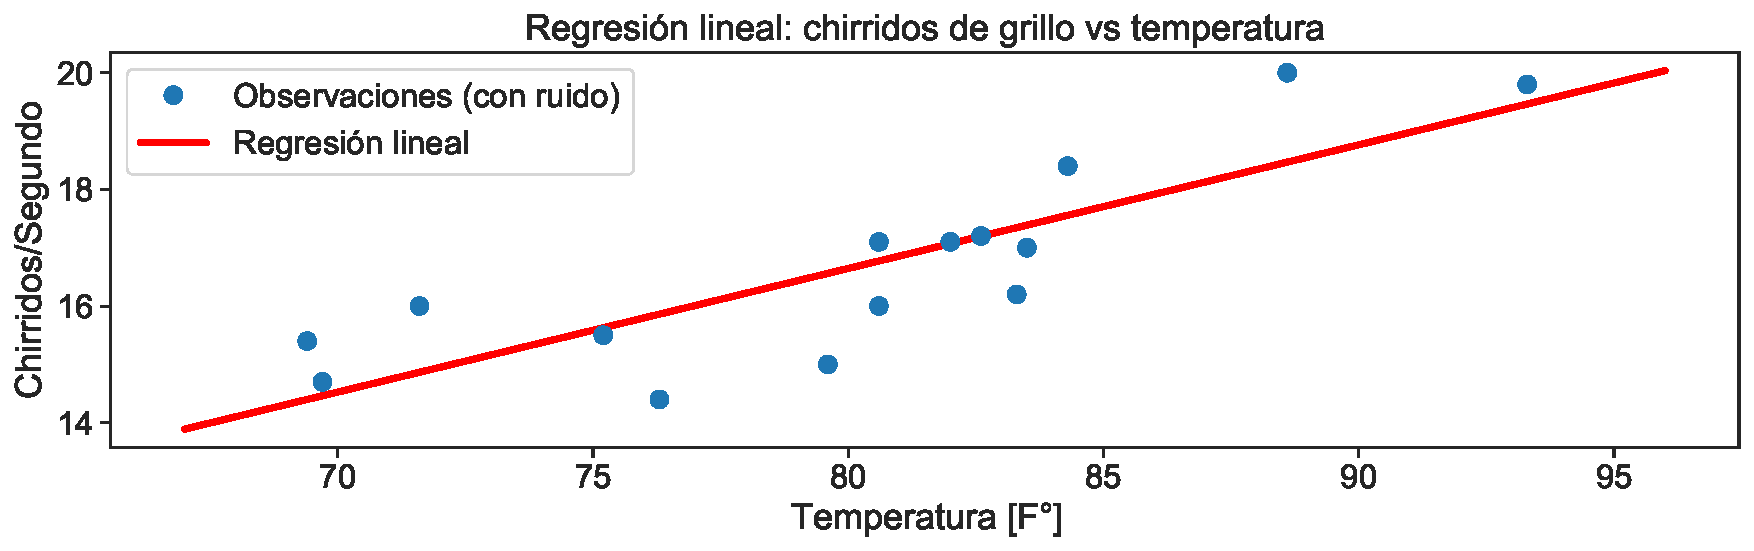
\includegraphics[width=0.7\textwidth]{../img/cap2_chirridos.pdf}\\
\end{figure}
	
\end{frame}

%Análisis de la solución de mínimos cuadrados.
\begin{frame}{Análisis de la solución de mínimos cuadrados}
Se obtuvo que el parámetro óptimo $\theta=(a,b)^\top$ corresponde a:
\begin{equation*}
	\theta = (\tX^\top\tX)^{-1}\tX^\top Y
\end{equation*}\pause

\begin{itemize}
	\item La expresión $\left(\tX^\top\tX \right)^{-1} \tX^\top$ corresponde a la pseudoinversa de Moore-Penrose de $\tX$.\pause
	\item Para que $\tX^\top\tX$ sea invertible, es necesario que $r(\tX)=M+1$.\pause
	\item Dado que $\tX\in\R^{N\times (M+1)}$, entonces $r(\tX)\leq\min\{N,M+1\}$ por lo que necesariamente se debe cumplir que $N\geq M+1$.\pause
	\item Es decir, el número de muestras debe ser mayor que el número de dimensiones. Intuitivamente esto se debe a que se necesitan $M+1$ puntos para fijar un hiperplano en $\R^{M+1}$
\end{itemize}
	
\end{frame}

%¿Por qué mínimos cuadrados?
\begin{frame}{¿Por qué mínimos cuadrados?}

Luego de haber encontrado el regresor óptimo de acuerdo al criterio de mínimos cuadrados, nace la pregunta de por qué utilizar ese criterio y no otro. Los principales argumentos son los siguiente: \pause

\begin{itemize}
	\item Su solución tiene forma cerrada, por lo que se evitan algoritmos numéricos.\pause
	\item Desde un punto interpretativo, el exponente 2 busca penalizar mayormente grandes diferencias (mayores que 1) entre la predicción y el valor real, mientras que le quita importancia a errores de predicción pequeños (menores que 1).\pause
	\item La medida del error cuadrático representa la varianza muestral: si considerásemos que $x_i$ e $y_i$ son observaciones iid de variables aleatorias $X$ e $Y$ respectivamente, entonces el error cuadrático medio asociado a la función $f$ definido por
\begin{equation*}
	ECM = \frac{1}{N}\sum_{i=1}^N (y_i-f(x_i))^2
\end{equation*}
corresponde a la varianza muestral de la variable aleatoria $Y-f(X)$ (asumiendo que $\E(Y-f(X))=0$).
\end{itemize}

\end{frame}

%Interpretación geométrica.
\begin{frame}{Interpretación geométrica}

El problema de regresión lineal requiere encontrar una solución aproximada de un sistema lineal sobredeterminado definido por 
\begin{equation*}
	\tX \theta = Y\label{eq:sist_lineal_sobredet}
\end{equation*}
donde la cantidad de incógnitas ($M+1$) es ampliamente superada por el número de ecuaciones ($N$), por lo que desde el punto de vista de un sistema lineal, la solución no necesariamente existe.\\~\ \pause

Por lo anterior, se puede proceder a encontrar la solución para $\theta$ que reporta \emph{la menor discrepancia} entre ambos lados de la ecuación \eqref{eq:sist_lineal_sobredet}, para esto, se realiza lo siguiente:\pause

\begin{itemize}
	\item Identificar el espacio formado por todos los posibles valores que toma la combinación lineal $\tX \theta$, es decir, el \emph{span} de todas las columnas de $\tX$:
	\begin{equation*}
		\text{span}(\tX) = \{\tX\theta:\theta\in\R^{M+1}\}\leq \R^N
	\end{equation*}\pause
	\item identificar el elemento de dicho espacio que está más cerca de $Y\in\R^N$  como la proyección del propio $Y$ en $\text{span}(\tX)$.
\end{itemize}

\end{frame}

%nterpretación geométrica.
\begin{frame}{Interpretación geométrica}

La condición para identificar dicha proyección es  precisamente que el vector error $e=Y-\tX \theta$ sea ortogonal al espacio  $\text{span}(\tX)$ generado por los datos de entrada. Dado que las columnas de $\tX$ son una base de $\text{span}(\tX)$:

\begin{equation*}
	u\in \text{span}(\tX) \iff \exists \theta_u\in \R^{M+1}: u=\tX\theta_u,
\end{equation*}\pause

por lo tanto:

\begin{columns}

\begin{column}{0.5\textwidth}

\begin{figure}[t]
	\centering
	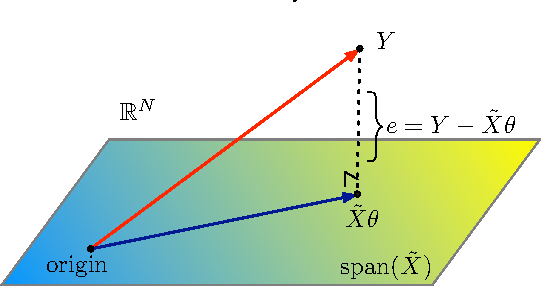
\includegraphics[width=\textwidth]{../img/cap2_intuicionLinReg.pdf}\\
	
	\label{fig:projection}
\end{figure}
	
\end{column}

\begin{column}{0.5\textwidth}


\begin{align*}
	 &e\perp \text{span}(\tX) \iff e\perp u,\forall u \in \text{span}(\tX)\\
	 & \iff (Y-\tX \theta)^\top \tX \theta_u = 0, \forall \theta_u \in \R^{M+1} \nonumber\\
	& \iff (Y-\tX \theta)^\top \tX=0\\
	& \iff  \theta = (\tX^\top\tX)^{-1}\tX^\top Y
\end{align*}

\end{column}

\end{columns} 

\pause Es decir, la distancia se minimiza para el $\theta$, correspondiente a la solución por mínimos cuadrados.
	
\end{frame}

%Problema de mínimos cuadrados.
\begin{frame}{Problema de mínimos cuadrados}

El principal problema del criterio de mínimos cuadrados es que es sensible a muestras atípicas (outliers) debido a la penalización cuadrática en su funcional de costos. Esto puede ser observado en la siguiente figura:

\begin{figure}[h]
	\centering
	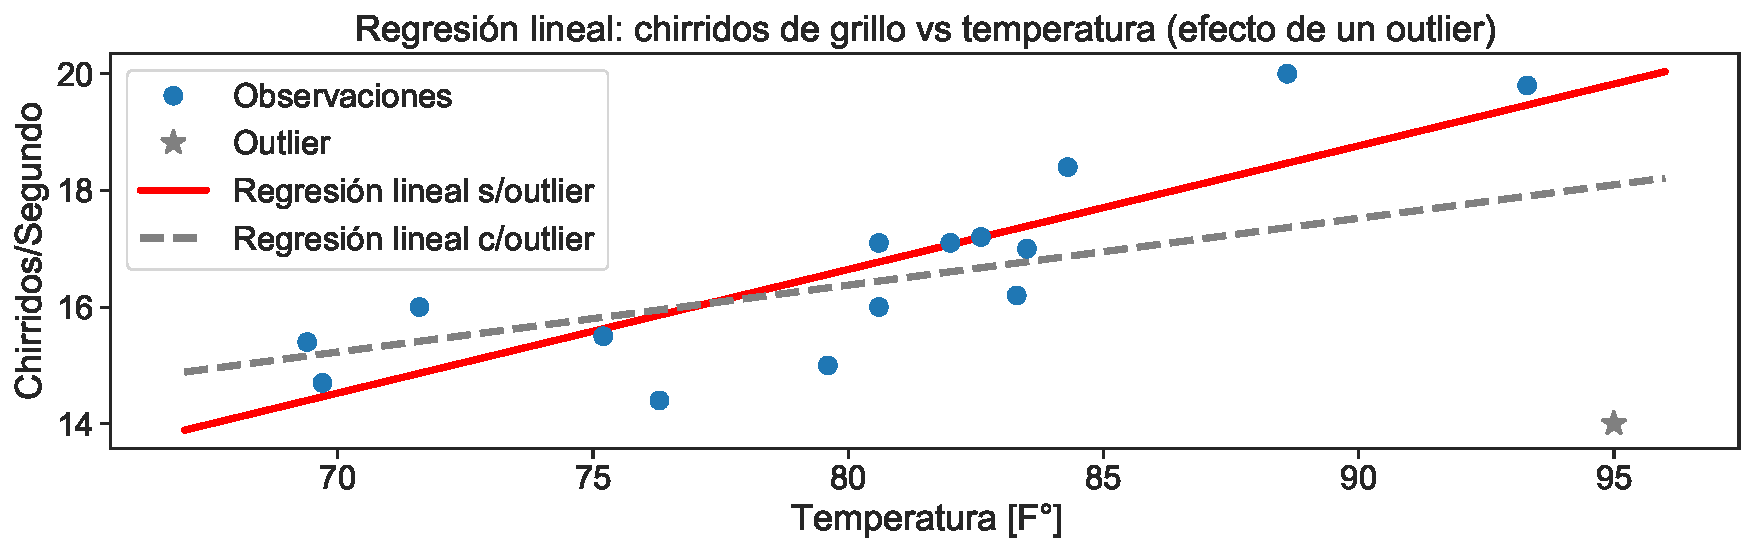
\includegraphics[width=1\textwidth]{../img/cap2_chirridos_outlier.pdf}\\
\end{figure} \pause

En conclusión, el criterio de mínimos cuadrados no es útil cuando existen muestras que se alejan de la tendencia buscada, por lo que se debe buscar algún método para corregir el problema. Una forma de realizar esto es \emph{mediante mínimos cuadrados regularizados}.
	
\end{frame}


\end{document}
